%!TeX root=./maximo.tex

\subsection{Torneio Cinético} \label{torneio:secao}
Considere o seguinte algoritmo para achar o valor máximo
em um conjunto de $n$ elementos: aloque um vetor \torneio~com
$2n - 1$ posições. Inicializamos as últimas $n$ posições com
os valores dos $n$ elementos e uma variável $i$ com o valor
da última posição, $i = 2n - 1$. Repita o seguinte processo
até que $i$ seja igual a $1$: se \torneio$[i] > $~\torneio$[i - 1]$,
então \torneio$\left[\floor{\frac{i}{2}}\right] =$~\torneio$[i]$,
caso contrário \torneio$\left[\floor{\frac{i}{2}}\right] =$~
\torneio$[i - 1]$, e, por fim, subtraia~$2$ de $i$. Dessa maneira,
ao fim da execução do algoritmo, em \torneio$[1]$ estará o maior
valor da coleção. Na verdade, podemos fazer a comparação de
maneira indireta, e guardar os índices dos elementos no vetor
\torneio~e não seus valores.

Podemos pensar nessas comparações entre \torneio$[i]$ e
\torneio$[i-1]$ como sendo partidas de um torneio classificatório,
por isso o nome torneio. Chamaremos de ``partida'' as comparações
entre \torneio$[i]$ e \torneio$[i-1]$ e diremos que o elemento~$j$
``vence'' o elemento $k$ quando os elementos $j$ e $k$ disputaram
uma partida entre si e o elemento $j$ possuía maior valor nesse
instante. Utilizaremos esse ``torneio'' para resolver o problema
do máximo cinético e, para implementá-lo, será utilizado um vetor
como o citado no algoritmo acima.
\begin{figure}[H]
    \centering
    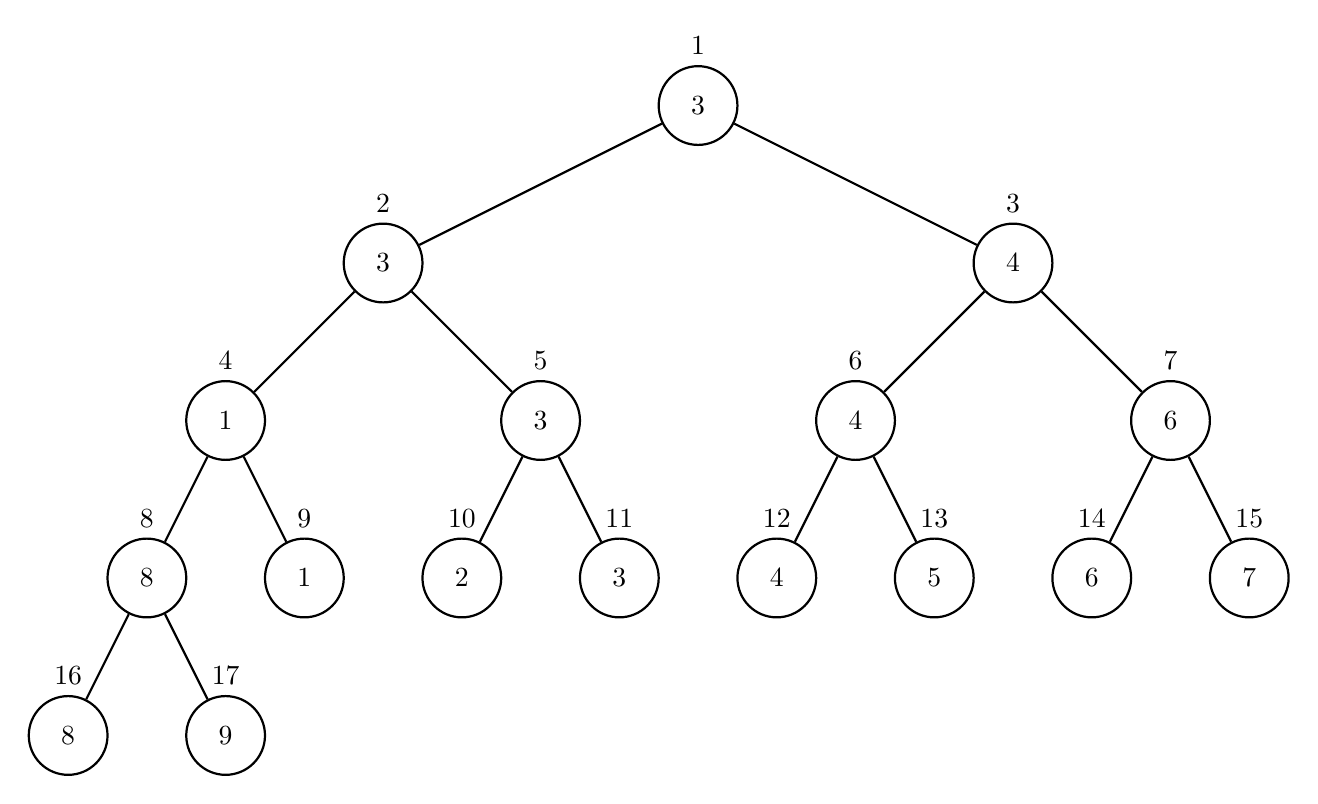
\begin{tikzpicture}[thick]
        \node[label={1},circle,draw,minimum size=1cm]
            (1) at (0,0) {$3$};
        \node[label={2},circle,draw,minimum size=1cm]
            (2) at (-4,-2) {$3$};
        \node[label={3},circle,draw,minimum size=1cm]
            (3) at (4,-2) {$4$};
        \node[label={4},circle,draw,minimum size=1cm]
            (4) at (-6,-4) {$1$};
        \node[label={5},circle,draw,minimum size=1cm]
            (5) at (-2,-4) {$3$};
        \node[label={6},circle,draw,minimum size=1cm]
            (6) at (2,-4) {$4$};
        \node[label={7},circle,draw,minimum size=1cm]
            (7) at (6,-4) {$6$};
        \node[label={8},circle,draw,minimum size=1cm]
            (8) at (-7,-6) {$8$};
        \node[label={9},circle,draw,minimum size=1cm]
            (9) at (-5,-6) {$1$};
        \node[label={10},circle,draw,minimum size=1cm]
            (10) at (-3,-6) {$2$};
        \node[label={11},circle,draw,minimum size=1cm]
            (11) at (-1,-6) {$3$};
        \node[label={12},circle,draw,minimum size=1cm]
            (12) at (1,-6) {$4$};
        \node[label={13},circle,draw,minimum size=1cm]
            (13) at (3,-6) {$5$};
        \node[label={14},circle,draw,minimum size=1cm]
            (14) at (5,-6) {$6$};
        \node[label={15},circle,draw,minimum size=1cm]
            (15) at (7,-6) {$7$};
        \node[label={16},circle,draw,minimum size=1cm]
            (16) at (-8,-8) {$8$};
        \node[label={17},circle,draw,minimum size=1cm]
            (17) at (-6,-8) {$9$};

        \draw[thick] (1) -- (2);
        \draw[thick] (2) -- (4);
        \draw[thick] (4) -- (8);
        \draw[thick] (4) -- (9);
        \draw[thick] (8) -- (16);
        \draw[thick] (8) -- (17);
        \draw[thick] (2) -- (5);
        \draw[thick] (5) -- (10);
        \draw[thick] (5) -- (11);
        \draw[thick] (1) -- (3);
        \draw[thick] (3) -- (6);
        \draw[thick] (3) -- (7);
        \draw[thick] (6) -- (12);
        \draw[thick] (6) -- (13);
        \draw[thick] (7) -- (14);
        \draw[thick] (7) -- (15);
    \end{tikzpicture}
    \caption{Torneio com $9$ elementos em que
    $3$ é o elemento com valor máximo.}
    \label{fig:torneio:exemplo}
\end{figure}
Inicialmente o vetor começa com os índices dos elementos
ocupando as últimas posições e construímos o torneio de
acordo com o valor de cada elemento no instante $t = 0$,
ou seja, com o valor $x_0$ de cada elemento.

Uma vez de posse do torneio montado, construímos um
certificado para cada elemento no torneio. O $i$-ésimo
certificado, que se refere ao par formado pelo $i$-ésimo
elemento da entrada e quem o venceu na última partida que
disputou, consiste no instante de tempo em que o $i$-ésimo
elemento passará a ter um valor maior que o valor do
elemento que o venceu anteriormente, se esse instante
for maior que o instante atual. Do contrário, o certificado
consiste em $+\infty$. % Esse valor do certificado é o seu \underline{prazo de validade}.

% Esses prazos de validade são os \underline{eventos} que causarão modificações no vetor que mantém os elementos ordenados pelo seu valor e consequentemente em alguns certificados.

É importante observar que o elemento que se encontra na
primeira posição do torneio não é vencido por ninguém no
instante \now. Dessa forma, sendo $i$ o elemento que ocupa
a primeira posição do torneio, associamos ao $i$-ésimo
certificado a chave $+\infty$.

\begin{figure}[H]
    \centering
    \begin{tikzpicture}[thick]
        \node[label={1},circle,draw,minimum size=1cm]
            (1) at (0,0) {$3$};
        \node[label={2},circle,draw,minimum size=1cm]
            (2) at (-4,-2) {$3$};
        \node[label={3},circle,draw,minimum size=1cm]
            (3) at (4,-2) {$4$};
        \node[label={4},circle,draw,minimum size=1cm]
            (4) at (-6,-4) {$1$};
        \node[label={5},circle,draw,minimum size=1cm]
            (5) at (-2,-4) {$3$};
        \node[label={6},circle,draw,minimum size=1cm]
            (6) at (2,-4) {$4$};
        \node[label={7},circle,draw,minimum size=1cm]
            (7) at (6,-4) {$6$};
        \node[label={8},circle,draw,minimum size=1cm]
            (8) at (-7,-6) {$8$};
        \node[label={9},circle,draw,minimum size=1cm]
            (9) at (-5,-6) {$1$};
        \node[label={10},circle,draw,minimum size=1cm]
            (10) at (-3,-6) {$2$};
        \node[label={11},circle,draw,minimum size=1cm]
            (11) at (-1,-6) {$3$};
        \node[label={12},circle,draw,minimum size=1cm]
            (12) at (1,-6) {$4$};
        \node[label={13},circle,draw,minimum size=1cm]
            (13) at (3,-6) {$5$};
        \node[label={14},circle,draw,minimum size=1cm]
            (14) at (5,-6) {$6$};
        \node[label={15},circle,draw,minimum size=1cm]
            (15) at (7,-6) {$7$};
        \node[label={16},circle,draw,minimum size=1cm]
            (16) at (-8,-8) {$8$};
        \node[label={17},circle,draw,minimum size=1cm]
            (17) at (-6,-8) {$9$};

        \draw[thick] (1) -- (2);
        \draw[<-, line width=\thickness, red] (2) -- (4);
        \draw[<-, line width=\thickness, red] (4) -- (8);
        \draw[thick] (4) -- (9);
        \draw[thick] (8) -- (16);
        \draw[<-, line width=\thickness, red] (8) -- (17);
        \draw[thick] (2) -- (5);
        \draw[<-, line width=\thickness, red] (5) -- (10);
        \draw[thick] (5) -- (11);
        \draw[<-, line width=\thickness, red] (1) -- (3);
        \draw[thick] (3) -- (6);
        \draw[<-, line width=\thickness, red] (3) -- (7);
        \draw[thick] (6) -- (12);
        \draw[<-, line width=\thickness, red] (6) -- (13);
        \draw[thick] (7) -- (14);
        \draw[<-, line width=\thickness, red] (7) -- (15);
    \end{tikzpicture}
    \caption{Torneio com 9 elementos e os certificados
    visualmente representados pelas setas vermelhas mais grossas.
    O certificado correspondente ao elemento 3 terá a
    chave~$+\infty$.}
    \label{fig:torneio:certificados}
\end{figure}

Esses $n$ certificados são colocados em uma fila de prioridade,
com o prazo de validade como chave. Estamos interessados nos
certificados com menor prazo de validade.

Para descrever a implementação das três operações,
precisamos estabelecer o nome das novas variáveis usadas.
São elas:
\begin{enumerate}
    % \item $n$: o número de elementos dados;
    % \item $x_0$ e \textit{speed}: vetores com o valor e a velocidade inicial de cada um dos $n$ elementos;
    % \item \now: instante atual;
    \item \torneio: vetor, de $2n - 1$ posições, com os
    índices dos $n$ elementos formando um torneio de acordo
    com o seu valor no instante \textit{now};

    \item \textit{cert}: vetor com os certificados;
    \textit{cert}$[i]$ guarda o certificado entre o elemento
    $i$ e quem o venceu na última partida que disputou, para
    $1 \leq i \leq n$;

    \item \textit{indT}: vetor de $n$ posições; \indt[$i$]
    guarda a posição em \torneio~em que $i$ perde uma partida,
    com $1 \leq i \leq n$. Se $i$ não perde nenhuma partida,
    \indt[$i$] é igual a $-1$.
    % \item \textit{Q}: fila de prioridade para os certificados.
\end{enumerate}

A interface da fila de prioridade que utilizaremos não se altera.

% Para implementar a operação updatePQ$(Q, i, t)$ em tempo logarítmico no número de elementos na fila de prioridade, é necessário utilizar um vetor adicional \textit{indQ} que guarda em \textit{indQ}$[i]$ a posição do $i$-ésimo certificado em $Q$.

% A operação advance$(t)$ não se altera, porém o tratamento de um evento sim. Um evento está associado a um certificado $(i, t)$ que expira no instante $t$. O tratamento do evento correspondente ao certificado $(i, t)$ consiste em trocar o valor da posição $\floor{\frac{j}{2}}$ do vetor \torneio~para $i$, sendo $j =$ \indt[$i$]. Após a troca é necessário recalcular o $k$-ésimo certficado, onde $k = 2\cdot \floor{\frac{j}{2}} + ((j + 1)~mod~2)$ é o irmão de $j$, além de atualizar \indt[\torneio[$k$]] para $k$. Depois de realizar essas operações definimos $j$ como $\floor{\frac{j}{2}}$ e repetimos o mesmo procedimento, só que dessa vez primeiro checamos se o valor do elemento na posição $j$ de \torneio~é maior ou igual a valor do elemento na posição $k$ de \torneio. Se $j$ se torna igual a $1$ ou se a checagem não for verdadeira paramos com as repetições e atualizamos \indt[\torneio[$j$]] para $j$.

% Finalmente, é necessário fazer ajustes em $Q$, alterando a chave dos certificados que sofreram alteração.
Na implementação da operação \textsc{event}, utilizaremos a rotina
\textsc{update}$(i)$ que calcula a nova validade $t$ do
elemento $j$ que se encontra na $i$-ésima posição
de \torneio, isto é, $j =~$\torneio[$i$]
certificado, se $1 \leq i \leq 2n - 1$, e chama a rotina
\textsc{updatePQ}$(Q, i, t)$.

\begin{algorithm}[H]
    \caption{Função \textsc{update}.} \label{torneio:update}
\begin{algorithmic}[1]
    \Function{update}{$i$}
        \If{$i = 1$}
            \State $t \leftarrow \infty$
        \EndIf
        \If{$1 < i \leq 2n - 1$}
            \State $t \leftarrow $
            \Call{expire}{\torneio$[\floor{\frac{i}{2}}]$,
            \torneio$[i]$}
        \EndIf
        \State $j \leftarrow$ \torneio$[i]$
        \State \Call{updatePQ}{$Q,j,t$}
    \EndFunction
    % \LineComment{\Call{expire}{$i,j$} calcula a validade do certificado entre os elementos $i$ e $j$}
\end{algorithmic}
\end{algorithm}

\begin{algorithm}[H]
    \caption{Função \textsc{event}.} \label{torneio:evento}
\begin{algorithmic}[1]
    \Function{event}{\null}
        \State $i \leftarrow  $ \Call{minPQ}{$Q$}
        \While{\cert[$i$] = \now}
            \State $j \leftarrow~$\indt[$i$]
            \State $k \leftarrow 2\cdot \floor{\frac{j}{2}} +
            ((j + 1)\mod2)$ \Comment{adversário}
            \While{$j > 1$ \AND \Call{value}{$j$} $\geq$
            \Call{value}{$k$}}
                \State \torneio[$\floor{\frac{j}{2}}$]
                $\leftarrow~$\torneio[$j$]
                \State \indt[\torneio[$k$]] $\leftarrow k$
                \State \Call{update}{$k$}
                \State $j \leftarrow \floor{\frac{j}{2}}$
                \State $k \leftarrow 2\cdot \floor{\frac{j}{2}}
                + ((j + 1)\mod2)$
            \EndWhile
            \State \indt[\torneio[$j$]] $\leftarrow j$
            \State \Call{update}{$j$}
            \State $i \leftarrow  $ \Call{minPQ}{$Q$}
        \EndWhile
            % \LineComment{swapHeap$(i, \floor{\frac{i}{2}})$ troca \heap[$i$] por \heap$\left[\floor{\frac{i}{2}}\right]$}
    \EndFunction
    \LineComment{\Call{value}{$j$} retorna \speed$[j]~\cdot$ \now + $x_0[j]$}
\end{algorithmic}
\end{algorithm}

No trecho das linhas $5$ - $11$ do código \ref{torneio:evento},
o resultado da partida entre o elemento~$j$ e seu adversário
que se encontra na posição $k$ de \torneio~é recalculado, e o
certificado correspondente é atualizado. Caso o resultado da
partida tenha sido alterado, a verificação se propaga para o
nível de cima.

\begin{figure}[H]
    \centering
    \begin{tikzpicture}[thick]
        \node[label={1},circle,draw,minimum size=1cm]
            (1) at (0,0) {$3$};
        \node[label={2},circle,draw,minimum size=1cm]
            (2) at (-4,-2) {$3$};
        \node[label={3},circle,draw,minimum size=1cm]
            (3) at (4,-2) {$4$};
        \node[label={4},circle,draw,minimum size=1cm]
            (4) at (-6,-4) {$1$};
        \node[label={5},circle,draw,minimum size=1cm]
            (5) at (-2,-4) {$3$};
        \node[label={6},circle,draw,minimum size=1cm]
            (6) at (2,-4) {$4$};
        \node[label={7},circle,draw,minimum size=1cm]
            (7) at (6,-4) {$6$};
        \node[label={8},circle,draw,minimum size=1cm]
            (8) at (-7,-6) {$8$};
        \node[label={9},circle,draw,minimum size=1cm]
            (9) at (-5,-6) {$1$};
        \node[label={10},circle,draw,minimum size=1cm]
            (10) at (-3,-6) {$2$};
        \node[label={11},circle,draw,minimum size=1cm]
            (11) at (-1,-6) {$3$};
        \node[label={12},circle,draw,minimum size=1cm]
            (12) at (1,-6) {$4$};
        \node[label={13},circle,draw,minimum size=1cm]
            (13) at (3,-6) {$5$};
        \node[label={14},circle,draw,minimum size=1cm]
            (14) at (5,-6) {$6$};
        \node[label={15},circle,draw,minimum size=1cm]
            (15) at (7,-6) {$7$};
        \node[label={16},circle,draw,minimum size=1cm]
            (16) at (-8,-8) {$8$};
        \node[label={17},circle,draw,minimum size=1cm]
            (17) at (-6,-8) {$9$};

        \draw[thick] (1) -- (2);
        \draw[<-,line width=\thickness, red] (2) -- (4);
        \draw[<-,thick, dashed, red] (4) -- (8);
        \draw[thick] (4) -- (9);
        \draw[thick] (8) -- (16);
        \draw[<-,line width=\thickness, red] (8) -- (17);
        \draw[thick] (2) -- (5);
        \draw[<-,line width=\thickness, red] (5) -- (10);
        \draw[thick] (5) -- (11);
        \draw[<-,line width=\thickness, red] (1) -- (3);
        \draw[thick] (3) -- (6);
        \draw[<-,line width=\thickness, red] (3) -- (7);
        \draw[thick] (6) -- (12);
        \draw[<-,line width=\thickness, red] (6) -- (13);
        \draw[thick] (7) -- (14);
        \draw[<-,line width=\thickness, red] (7) -- (15);
    \end{tikzpicture}
    \caption{cert[$8$] expirou.}
    \label{fig:torneio:evento}
\end{figure}

\begin{figure}[H]
    \centering
    \begin{tikzpicture}[thick]
        \node[label={1},circle,draw,minimum size=1cm]
            (1) at (0,0) {$8$};
        \node[label={2},circle,draw,minimum size=1cm]
            (2) at (-4,-2) {$8$};
        \node[label={3},circle,draw,minimum size=1cm]
            (3) at (4,-2) {$4$};
        \node[label={4},circle,draw,minimum size=1cm]
            (4) at (-6,-4) {$8$};
        \node[label={5},circle,draw,minimum size=1cm]
            (5) at (-2,-4) {$3$};
        \node[label={6},circle,draw,minimum size=1cm]
            (6) at (2,-4) {$4$};
        \node[label={7},circle,draw,minimum size=1cm]
            (7) at (6,-4) {$6$};
        \node[label={8},circle,draw,minimum size=1cm]
            (8) at (-7,-6) {$8$};
        \node[label={9},circle,draw,minimum size=1cm]
            (9) at (-5,-6) {$1$};
        \node[label={10},circle,draw,minimum size=1cm]
            (10) at (-3,-6) {$2$};
        \node[label={11},circle,draw,minimum size=1cm]
            (11) at (-1,-6) {$3$};
        \node[label={12},circle,draw,minimum size=1cm]
            (12) at (1,-6) {$4$};
        \node[label={13},circle,draw,minimum size=1cm]
            (13) at (3,-6) {$5$};
        \node[label={14},circle,draw,minimum size=1cm]
            (14) at (5,-6) {$6$};
        \node[label={15},circle,draw,minimum size=1cm]
            (15) at (7,-6) {$7$};
        \node[label={16},circle,draw,minimum size=1cm]
            (16) at (-8,-8) {$8$};
        \node[label={17},circle,draw,minimum size=1cm]
            (17) at (-6,-8) {$9$};

        \draw[thick] (1) -- (2);
        \draw[thick] (2) -- (4);
        \draw[thick] (4) -- (8);
        \draw[<-,thick, dashdotted, blue] (4) -- (9);
        \draw[thick] (8) -- (16);
        \draw[<-,line width=\thickness, red] (8) -- (17);
        \draw[<-,thick, dashdotted, blue] (2) -- (5);
        \draw[<-,line width=\thickness, red] (5) -- (10);
        \draw[thick] (5) -- (11);
        \draw[<-,thick, dashdotted, blue] (1) -- (3);
        \draw[thick] (3) -- (6);
        \draw[<-,line width=\thickness, red] (3) -- (7);
        \draw[thick] (6) -- (12);
        \draw[<-,line width=\thickness, red] (6) -- (13);
        \draw[thick] (7) -- (14);
        \draw[<-,line width=\thickness, red] (7) -- (15);
    \end{tikzpicture}
    \caption{Após \cert[$8$] ter expirado, o elemento
    $8$ passou a vencer o elemento $1$ e \torneio[$4$] foi
    atualizado, o elemento $8$ também venceu dos elementos
    $3$ e $4$ e \torneio[$2$] e \torneio[$1$] foram atualizados.
    Os certificados \cert[$1$], \cert[$3$] e \cert[$4$],
    indicados pelas setas azuis, também foram atualizados}
    \label{fig:predeventtorn}
\end{figure}

A operação \textsc{query\_max}$()$ consiste em devolver
\torneio$[1]$, enquanto que a operação \textsc{change}$(j, v)$
consiste em alterar a posição $x_0[j]$ para
$x_0[j] + (\mathit{speed}[j] - v)\cdot now$, a posição
\textit{speed}$[j]$ para \textit{v} e recalcular os eventuais
certificados de que $j$ participa. Para tanto, a partir
da posição $i$ em que $j$ se encontra no vetor \torneio,
podemos recalcular \textit{cert}$[j]$ e então continuamos
visitando as partidas em que $j$ participou para atualizar
os certificados daqueles que perderam de $j$, acionando a
rotina \textsc{updatePQ} para fazer os devidos acertos em
$Q$ correspondentes a estas modificações.
$\\$

\begin{algorithm}[H]
    \caption{Função \textsc{query\_max}.} \label{torn:advance}
\begin{algorithmic}[1]
    \Function{query\_max}{\null}
        \State \Return \torneio$[1]$
    \EndFunction
\end{algorithmic}
\end{algorithm}

\begin{algorithm}[H]
    \caption{Função \textsc{change}.} \label{torn:change}
\begin{algorithmic}[1]
    \Function{change}{$j, v$}
        \State $x_0$[$j$] $\leftarrow x_0$[$j$]
        $+~($\speed[$j$] $-~v)~\cdot~$\now;
        \State \speed[$j$] $\leftarrow v$
        \State $i \leftarrow $ \indt[$j$]
        \State \Call{update}{$i$}
        \While{$i < n$}
            \If{$\torneio[i] = \torneio[2i]$}
                \State $i \leftarrow 2i$
            \Else
                \State $i \leftarrow 2i + 1$
            \EndIf
            \State $k \leftarrow 2\cdot \floor{\frac{i}{2}}
            + ((i + 1)\mod2)$ \Comment{adversário}
            \State \Call{update}{$k$}
        \EndWhile
    \EndFunction
\end{algorithmic}
\end{algorithm}
\begin{figure}[H]
    \centering
    \begin{tikzpicture}[thick]
        \node[label={1},circle,draw,minimum size=1cm]
            (1) at (0,0) {$3$};
        \node[label={2},circle,draw,minimum size=1cm]
            (2) at (-4,-2) {$3$};
        \node[label={3},circle,draw,minimum size=1cm]
            (3) at (4,-2) {$4$};
        \node[label={4},circle,draw,minimum size=1cm]
            (4) at (-6,-4) {$1$};
        \node[label={5},circle,draw,minimum size=1cm]
            (5) at (-2,-4) {$3$};
        \node[label={6},circle,draw,minimum size=1cm]
            (6) at (2,-4) {$4$};
        \node[label={7},circle,draw,minimum size=1cm]
            (7) at (6,-4) {$6$};
        \node[label={8},circle,draw,minimum size=1cm]
            (8) at (-7,-6) {$8$};
        \node[label={9},circle,draw,minimum size=1cm]
            (9) at (-5,-6) {$1$};
        \node[label={10},circle,draw,minimum size=1cm]
            (10) at (-3,-6) {$2$};
        \node[label={11},circle,draw,minimum size=1cm]
            (11) at (-1,-6) {$3$};
        \node[label={12},circle,draw,minimum size=1cm]
            (12) at (1,-6) {$4$};
        \node[label={13},circle,draw,minimum size=1cm]
            (13) at (3,-6) {$5$};
        \node[label={14},circle,draw,minimum size=1cm]
            (14) at (5,-6) {$6$};
        \node[label={15},circle,draw,minimum size=1cm]
            (15) at (7,-6) {$7$};
        \node[label={16},circle,draw,minimum size=1cm]
            (16) at (-8,-8) {$8$};
        \node[label={17},circle,draw,minimum size=1cm]
            (17) at (-6,-8) {$9$};

        \draw[thick] (1) -- (2);
        \draw[<-,thick, dashdotted, blue] (2) -- (4);
        \draw[<-,line width=\thickness, red] (4) -- (8);
        \draw[thick] (4) -- (9);
        \draw[thick] (8) -- (16);
        \draw[<-,line width=\thickness, red] (8) -- (17);
        \draw[thick] (2) -- (5);
        \draw[<-,thick, dashdotted, blue] (5) -- (10);
        \draw[thick] (5) -- (11);
        \draw[<-,thick, dashdotted, blue] (1) -- (3);
        \draw[thick] (3) -- (6);
        \draw[<-,line width=\thickness, red] (3) -- (7);
        \draw[thick] (6) -- (12);
        \draw[<-,line width=\thickness, red] (6) -- (13);
        \draw[thick] (7) -- (14);
        \draw[<-,line width=\thickness, red] (7) -- (15);
    \end{tikzpicture}
    \caption{Após atualizar a velocidade do elemento $3$,
    \cert[$2$], \cert[$1$] e \cert[$4$] foram atualizados
    porque disputaram partidas com $3$.}
    \label{fig:torneio:change}
\end{figure}